\newif\ifpagetuning

\pagetuningtrue % trying to get page breaks in the best spots

\newif\ifnotcutting \notcuttingfalse % set if not cutting down to size

\newif\iffinaldraft \finaldrafttrue % true if it's the final version

\newif\iftimestamp\timestamptrue  % show MD5 stamp of paper

% \timestampfalse % it's post-submission time


\IfFileExists{timestamp.tex}{}{\timestampfalse}

 \newif\ifpdfmadness

\ifx\pdfoutput\undefined
   \pdfmadnessfalse
\else
   \ifnum\pdfoutput=1
     \pdfmadnesstrue
   \else
     \pdfmadnessfalse
   \fi
\fi

\documentclass[nonatbib,preprint,blockstyle,times]{sigplanconf}
  % at 9pt anything but block style is unreadable

\newcommand\mrfy{MRFy} % damn you Noah

\newcommand\txprobj[3][]{a#1_{{#2}_{j-1}{#3}_j}}
\newcommand\txprobjj[3][]{a#1_{{#2}_{j-1}{#3}_j}}
\newcommand\alignwidth{\ensuremath C} % number of columns in an alignment
\newcommand\pairedwith[1]{{\pi(#1)}}

\newcommand\primcons{\texttt{\small(:)}}

\ifpagetuning
  \newcommand\tuningbox{\vbox}
\else
  \newcomming\tuningbox{\relax}
\fi

\newcommand\naive{na\"\i ve}
\usepackage{url}
\usepackage{amsmath}
\usepackage{array}
\usepackage{listings}
\usepackage{graphicx}
\lstset{
    tabsize = 2,
    basicstyle = \ttfamily,
    language = Haskell
    }    

\newcommand\figref[1]{Figure~\ref{#1}}
\newcommand\secref[1]{Section~\ref{sec:#1}}
\newcommand\seclabel[1]{\label{sec:#1}}

\usepackage{verbatim}

\newif\ifverbatimsmall
\verbatimsmallfalse
\makeatletter
\def\verbatim@font{%
   \normalfont\ttfamily
   \ifverbatimsmall\small\fi
   \hyphenchar\font\m@ne
   \@noligs}
\makeatother

\newenvironment{smallverbatim}{\par\small\verbatimsmalltrue\verbatim}{\endverbatim}
\newcommand\smallverbatiminput[1]{%
  \everypar=\expandafter{\the\everypar
       \verbatimsmallfalse
%       \belowdisplayskip=\abovedisplayskip
%       \belowdisplayshortskip=\abovedisplayshortskip
       \topsep=\standardvspace}%
  \topsep=0.78\topsep
%  \belowdisplayskip=0.78\belowdisplayskip
%  \belowdisplayshortskip=0.78\belowdisplayshortskip
  \verbatimsmalltrue\verbatiminput{#1}}
\newcommand\smallverbatiminputx[1]{\vspace*{-8pt}{\small\verbatiminput{#1}}} % WTF?? {\LaTeX} hell
\newcommand\smallfuzzverbatiminput[2]{%
  \everypar\expandafter{\the\everypar\hfuzz=0pt\relax}%
  \hfuzz=#1 \smallverbatiminput{#2}}

\renewcommand\ttdefault{aett}

  \long\def\remark#1{%
      \ifvmode
         \marginpar{\raggedright\hbadness=10000
         \parindent=8pt \parskip=2pt
         \def\baselinestretch{0.8}\tiny
         \itshape\noindent #1\par}%
      \else
          \unskip\raisebox{-3.5pt}{\rlap{$\scriptstyle\diamond$}}%
          \marginpar{\raggedright\hbadness=10000
         \parindent=8pt \parskip=2pt
         \def\baselinestretch{0.8}\tiny
         \itshape\noindent #1\par}%
      \fi}

\iffinaldraft
  \newcommand\finalremark{\remark}
\else
  \newcommand\finalremark[1]{\relax}
\fi

\usepackage[authoryear]{natbib}
\bibpunct();A{},
\let\cite\citep
\let\citeyearnopar=\citeyear
\let\citeyear=\citeyearpar



\IfFileExists{timestamp.tex}{\input{timestamp}}{}
\renewcommand{\floatpagefraction}{0.9} % must be less than \topfraction
\renewcommand{\topfraction}{0.95}
\renewcommand{\textfraction}{0.05}


\begin{document}
\parskip=0.9\parskip % cheating
\advance \parskip by 0pt plus 0.1pt

\overfullrule=10pt


\conferenceinfo{ICFP'12,} {September 9--15, 2012, Copenhagen, Denmark.}
\CopyrightYear{2012}
\copyrightdata{978-1-4503-1054-3/12/09}

%\titlebanner{banner above paper title}        % These are ignored unless
\preprintfooter{Haskell in Computational Biology}   % 'preprint' option specified.
\iftimestamp
\preprintfooter{\mdfivestamp} 
\fi

\title{Experience Report: Haskell in Computational Biology}
% \subtitle{Subtitle Text, if any}


\authorinfo{Noah M. Daniels \and Andrew Gallant \and Norman Ramsey}
           {Department of Computer Science, Tufts University}
           {{\rmfamily\{}ndaniels, agallant, nr{\rmfamily\}}@cs.tufts.edu}


\maketitle

%
% It can't hurt to remind everyone involved exactly what an Experience
% Report is.
%
%
\begin{abstract}
%An Experience Report provides {evidence} that functional
%programming really works, or it describes obstacles that prevent
%functional programming from working.   
Haskell gives computational biologists
the flexibility and rapid prototyping of a scripting
language, plus the performance of native code.
In~our experience, higher-order functions, lazy evaluation, and
monads really worked, but
profiling and debugging presented obstacles.
Also, Haskell libraries vary greatly:
memoization combinators and parallel-evaluation
strategies helped us a lot,
but other, nameless libraries mostly got in our way.
Despite the obstacles and the uncertain quality of some libraries,
Haskell's ecosystem
made it easy for us to develop new algorithms in computational
biology.
\end{abstract}

\category{D.1.1}{Applicative (Functional) Programming}{}
\category{J.3}{Biology and genetics}{}
% \category{CR-number}{subcategory}{third-level}
% 
% \terms
% term1, term2
% 
% \keywords
% keyword1, keyword2

\section{Introduction}

Computational biologists write software that answers questions about 
sequences of nucleic acids (genomic data) or sequences of amino 
acids (proteomic data). 
When performance is paramount,
software is usually written in C~or~C++. 
When convenience, readability, and
productivity are more important,
software is usually written in a dynamically typed
or domain-specific language like
Perl, Python, Ruby, SPSS, or~R.
In~this paper, we report on experience using a third kind of language,
Haskell: 
\begin{itemize}
\item
We had to reimplement an
algorithm already implemented in~C++, 
and the Haskell code is slower.
But the Haskell code was easy to write,     % coherent subject!
it is clearly connected to the underlying
algorithm (\secref{viterbi}),
it was easy to parallelize,
and it performs well enough
(\secref{perf}).
\ifpagetuning
And overall,
\else
Moreover, measured as a whole, 
\fi
the software that incorporates our new
code 
performs significantly
better than the~C++ software that preceded~it.
\item
Higher-order functions made it unusually easy to
create and experiment with new stochastic-search algorithms
(\secref{hofs}).
\item
Haskell slowed us down in only one area:  understanding and
improving
performance (\secref{awkward-profiling}).
%%  \item
%%  The only significant impediment that Haskell presented to our
%%  research was the difficulty of understanding and improving the
%%  performance of Haskell programs (\secref{awkward-profiling}).
\item
Although the first two authors are computational
biologists with little background in functional programming,
Haskell has made it easy for us to explore new research ideas.
By~contrast,
our group's C++ code has not
made it easy to explore
% been a good vehicle for exploring 
new ideas
(\secref{comparo}).
\item
The Haskell community offers libraries and tools that
promise powerful abstractions.
Some kept the promise, saved us lots of effort, and were a pleasure
to~use.
Others, not so much.
And~we couldn't tell in advance which 
\ifpagetuning
would be which
\else
experience we were likely to have
\fi
 (\secref{penumbra}).
\looseness=-1
\end{itemize}




\section{The biology}

Proteins %%% are cellular machinery. They
interact with one another and with other 
molecules to carry out the functions of living cells: metabolism, regulation, 
signaling, and so on.
A~protein's function is determined by its structure, 
and its structure is determined by the sequence of amino acids that
form the protein.
The amino-acid sequence is ultimately determined by a sequence of
nucleic acids in DNA, which we call a gene.
Given a genetic sequence, biologists wish to know the cellular
function of the protein that gene codes for.
One of the best known methods of discovering such function is
to find other proteins of 
similar structure, which likely share similar function.
Proteins that share structure and function are expected to be
descended from a common ancestor---in biological terms, \emph{homologous}---and
thus
the problem of identifying proteins similar to a \textit{query sequence} is called 
\textit{homology detection}.




Computational biologists detect homologies by building 
algorithms which, given a {query sequence}, %% of amino acids,
find known proteins of similar structure.
When similar proteins are formed from amino-acid sequences that
are not too different from the query sequence, the homology can be
detected by
a family of algorithms called 
\textit{hidden Markov models}~\cite{Eddy:1998ut}.
But in real biological systems,
proteins with similar structure and function may be formed from significantly 
different amino-acid sequences, which are not close in edit distance.
Our~research software, MRFy (pronounced
``Murphy''), can detect homologies 
in amino-acid sequences that are only distantly related.
MRFy is available at \url{mrfy.cs.tufts.edu}.
%
%We will explain an 
%algorithm for detecting reasonably similar sequences, and then move on to 
%explain MRFy, our novel approach for detecting more distantly related sequences 
%for proteins that share similar structure and function.
%

%
% I hope the new intro renders these two sentences unnecessary. ---NR
%
%
%%  
%%  To~enable you to understand our experience with Haskell,
%%  we~sketch not only the MRFy algorithm (\secref{mrfy})
%%  but also one of the older hidden-Markov algorithms (\secref{viterbi}),
%%  which is incorporated into~MRFy.


\section{The software}



Homology-detection software is most often used in one of two ways:
to test a hypothesis about 
the function of a single, newly discovered protein, or 
to compare every protein in a genome against a library of known protein 
structures.
Either way, 
the software is \emph{trained}
on a group of proteins that share function and structure.
These proteins are identified by a biologist, who puts
their amino-acid sequences into an
\emph{alignment}. 
This alignment relates individual amino acids in a set of homologous proteins.
An~alignment may be represented as a matrix
in which each row corresponds to the amino-acid sequence of a protein,
and each column groups amino acids that play similar roles in
different proteins (Figure~\ref{alignment}).


An alignment may contain \emph{gaps}, which in 
\figref{alignment} are shown as dashes.
A~gap in row~2, column~$j$ indicates that as proteins evolved, either 
protein~2 lost its amino acid in position~$j$, or 
other proteins gained an amino acid in position~$j$.
If~column~$j$ contains few gaps, 
it~is considered a \emph{consensus column},
and the few proteins with gaps probably lost amino acids via
\emph{deletions}.
%%  \remark{NMD: Missing is the fact that all these models
%%  are directionless; they don't care whether something was gained or lost
%%  over time. But this doesn't matter.}
If~column~$j$ contains \emph{mostly} gaps, 
it~is considered a \emph{non-consensus column},
and the few proteins without gaps probably gained amino acids via
\emph{insertions}. 

Once a protein alignment is constructed, it~is used to train a
\emph{hidden Markov model}. 
A~hidden Markov model is a probabilistic finite-state machine which 
can assign a probability to any query sequence.
A~protein whose query sequence has a higher probability is more likely to %
be homologous to the proteins in the alignment.
We~write a query sequence as $x_1, \ldots, x_{\scriptscriptstyle N}$,
where each $x_i$~is 
an amino acid.
$N$~need not be the same as the number of columns in the alignment,
which we write~\alignwidth.


\begin{figure}
\ifpdfmadness
\centerline{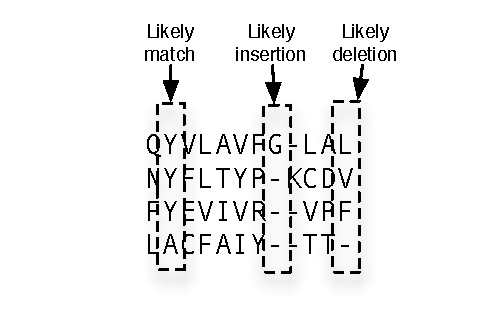
\includegraphics[width=6cm]{alignment.pdf}} 
\else
\centerline{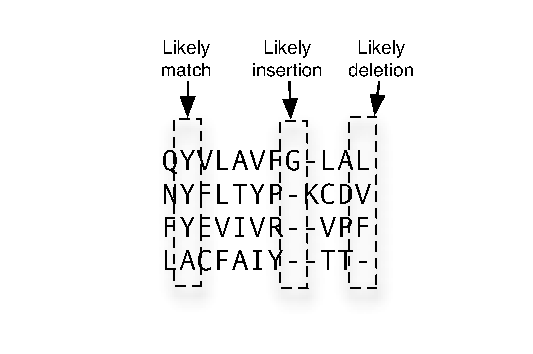
\includegraphics[width=6cm]{alignment.eps}} 
\fi

\caption{A~structural alignment of four proteins $(\alignwidth = 12)$}
\label{alignment} 
\end{figure}



A~hidden Markov model carries probabilities on some states and on all
state transitions.
Both the probabilities and the states are determined by the alignment:
\begin{itemize}
\item
For each column~$j$ of the alignment, the hidden Markov model has a
\emph{match state}~$M_j$.
The match state contains a table $e_{M_j}(x)$ which gives the
 probability that a homologous protein has amino acid~$x$ in
 column~$j$.
\item 
For each column~$j$ of the alignment, the hidden Markov model has an
\emph{insertion state}~$I_j$.
The insertion state contains a table $e_{I_j}(x)$ which gives the
probability that a homologous protein has gained amino acid~$x$ by
insertion at column~$j$.
\item
For each column~$j$ of the alignment, the hidden Markov model has a
\emph{deletion state}~$D_j$.
The deletion state determines the probability that a homologous protein
has lost an amino acid by deletion from column~$j$.
\end{itemize}
The probabilities $e_{M_j}(x)$ and $e_{I_j}(x)$ are \emph{emission probabilities}.

A hidden Markov model also has distinguished \emph{Begin} and \emph{End} states.
In~our representation, each state contains a probability or a table of
probabilities, and it is also labeled with one of these labels:
\smallverbatiminput{statelabel}


We~use the ``Plan7'' hidden Markov model, which forbids direct
transitions between insertion 
states and deletion states \cite{Eddy:1998ut}. 
The model gets its name because there are exactly
seven possible transitions
into the states of any column~$j$.
Each transition has its own probability:
\begin{itemize} 
\item
A~transition into a match state 
is more likely when column~$j$ is a consensus column.
Depending on the predecessor state, 
the probability of such a transition is 
$\txprobj M M$, $\txprobj I M$, or~$\txprobj D M$.
\item
A~transition into a deletion state 
is more likely when column~$j$ is a non-consensus column.
The probability of such a transition is 
$\txprobj M D$~or~$\txprobj D D$.
\item
A~transition into an insertion state 
is more likely when column~$j$ is a non-consensus column.
The probability of such a transition is 
$\txprobjj M I$~or~$\txprobjj I I$.
\end{itemize}



\begin{figure} 
\ifpdfmadness
\centerline{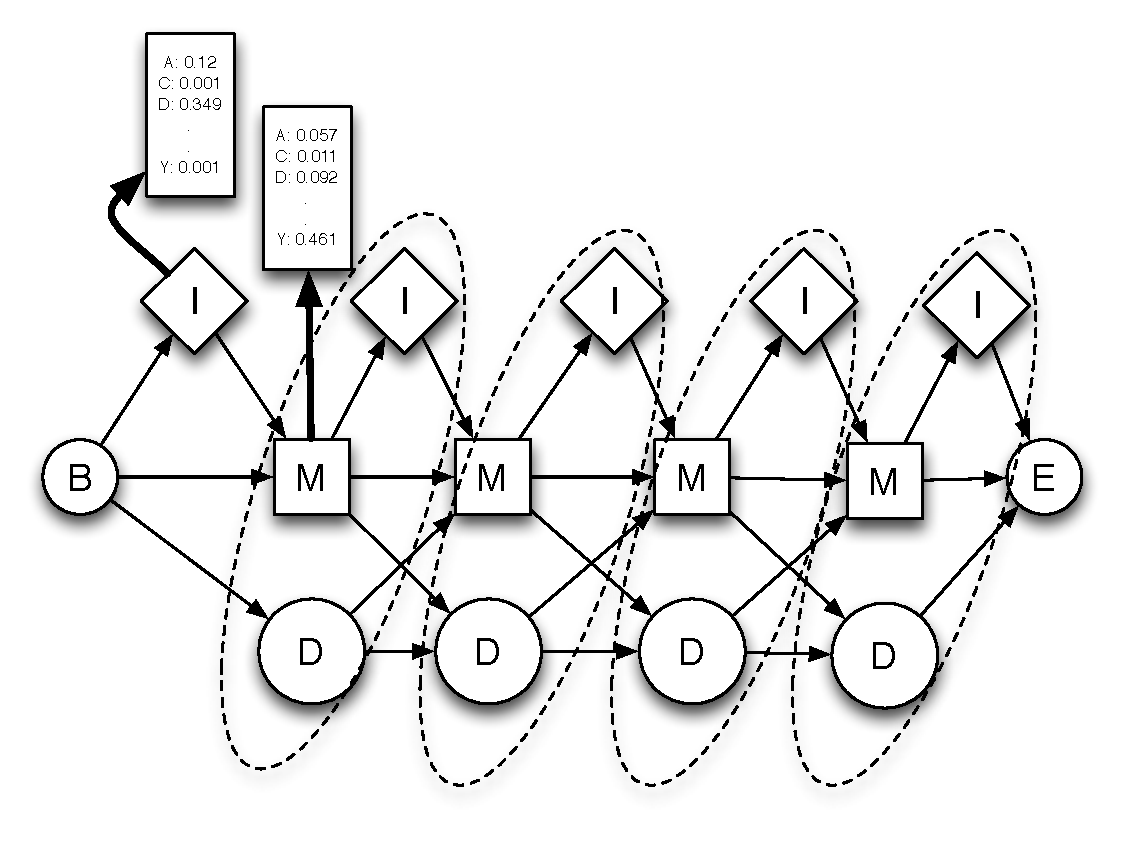
\includegraphics[width=8cm]{Plan7.pdf}} 
\else
\centerline{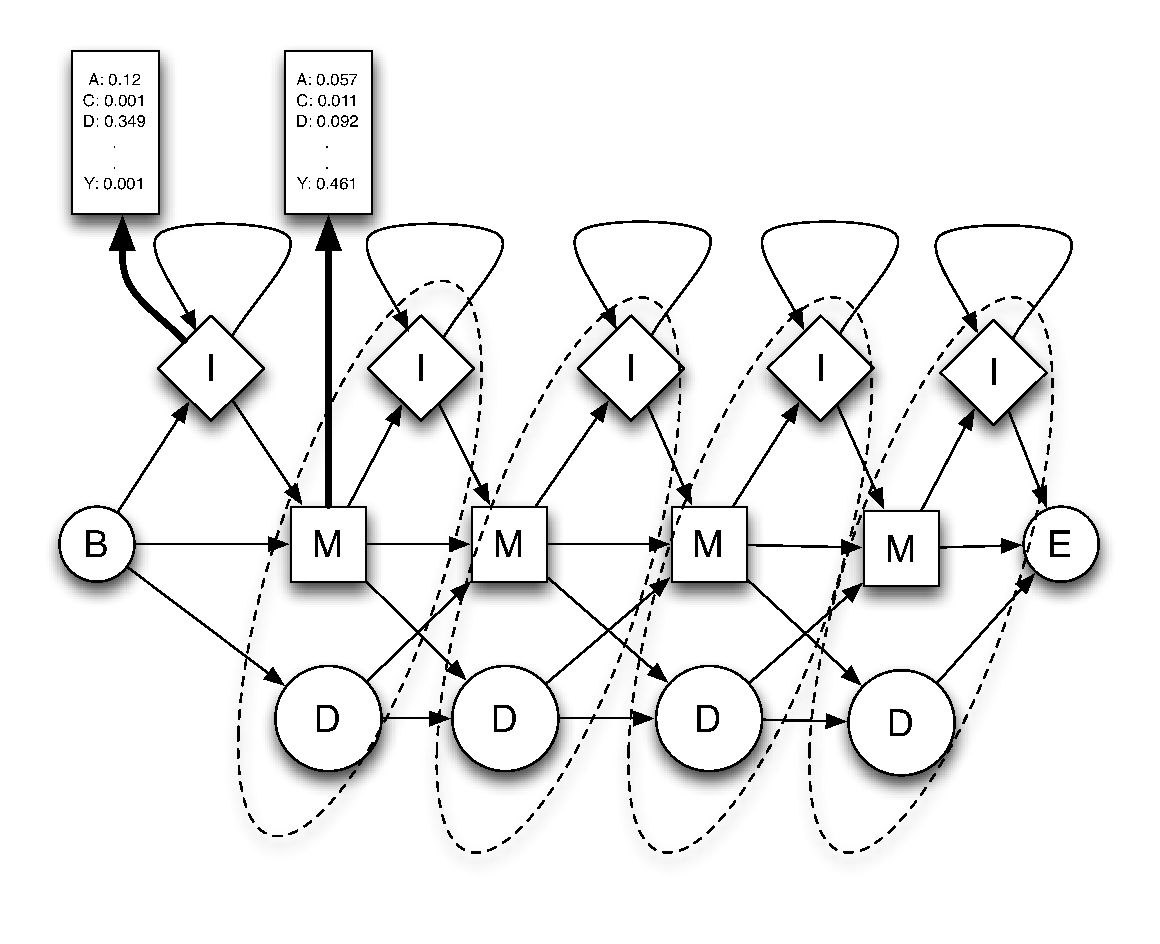
\includegraphics[width=8cm]{Plan7.eps}} 
\fi


This model
has begin and end states $B$~and~$E$,
as well as four
nodes, each containing 
an insertion state~$I$, 
a match state~$M$, and a
deletion state~$D$.

\caption{A hidden Markov model $(\alignwidth = 4)$}

\label{plan7} \end{figure}



\begin{figure*}
\newcommand\vsum[2]{#2&{}+{}& #1}

\def\goo{18pt}
\def\gum{14pt}
\[
\def\maxiquad{\hskip 1.2em\relax}
%\mskip -5mu
\begin{array}{@{}l@{}c@{}l}
V_{j}^{M}(i) &{}={}& \log\frac{e_{M_{j}}(x_{i})}{q_{x_{i}}} + \max \left\{
  \begin{array}{l@{}c@{}l}
  \vsum{V_{j-1}^{M}(i - 1)} {\log a_{M_{j-1}M_{j}}}\\
  \vsum{V_{j-1}^{I}(i - 1)} {\log a_{I_{j-1}M_{j}}}\\
  \vsum{V_{j-1}^{D}(i - 1)} {\log a_{D_{j-1}M_{j}}}\\
  \end{array} \right.\\[\goo]
V_{j}^{I}(i) &=& \log\frac{e_{I_{j}}(x_{i})}{q_{x_{i}}} + \max \left\{
  \begin{array}{l@{}c@{}l}
  \vsum{V_{j}^{M}(i - 1)} {\log a_{M_{j}I_{j}}}\\
  \vsum{V_{j}^{I}(i - 1)} {\log a_{I_{j}I_{j}}}\\
  \end{array} \right.\\[\gum]
V_{j}^{D}(i) &=& \max \left\{
  \begin{array}{l@{}c@{}l}
  \vsum{V_{j-1}^{M}(i)} {\log a_{M_{j-1}D_{j}}}\\
  \vsum{V_{j-1}^{D}(i)} {\log a_{D_{j-1}D_{j}}}\\
  \end{array} \right.\\
\end{array}
%
\hskip 1.5em\relax % \qquad too big
%
\begin{array}{l@{}c@{}l@{}}
V_{j}^{\prime M}(i) &{}={}& e^{\prime}_{M_{j}}(x_{i}) + \min \left\{
  \begin{array}{l@{}c@{}l}
  \vsum{V_{j-1}^{\prime M}(i - 1)} {a^{\prime}_{M_{j-1}M_{j}}}\\
  \vsum{V_{j-1}^{\prime I}(i - 1)} {a^{\prime}_{I_{j-1}M_{j}}}\\
  \vsum{V_{j-1}^{\prime D}(i - 1)} {a^{\prime}_{D_{j-1}M_{j}}}\\
  \end{array} \right.\\[\goo]
V_{j}^{\prime I}(i) &=& e^{\prime}_{I_{j}}(x_{i}) + \min \left\{
  \begin{array}{l@{}c@{}l}
  \vsum{V_{j}^{\prime M}(i - 1)} {a^{\prime}_{M_{j}I_{j}}}\\
  \vsum{V_{j}^{\prime I}(i - 1)} {a^{\prime}_{I_{j}I_{j}}}\\
  \end{array} \right.\\[\gum]
V_{j}^{\prime D}(i) &=& \min \left\{
  \begin{array}{l@{}c@{}l}
  \vsum{V_{j-1}^{\prime M}(i)} {a^{\prime}_{M_{j-1}D_{j}}}\\
  \vsum{V_{j-1}^{\prime D}(i)} {a^{\prime}_{D_{j-1}D_{j}}}\\
  \end{array} \right.\\[\gum]
%
\multicolumn3{l@{}}{%
  a'_{s \hat{s}} = - \log a_{s \hat{s}} 
\qquad
  e^{\prime}_{s}(x) = - \log\frac{e_{s}(x)}{q_{x}}
\qquad
  V_j^{\prime M}(i) = - V_j^{M}(i)
}
\\
\end{array}
%\mskip -5mu
\]

\caption{Viterbi's equations, in original and negated forms}
\label{viterbi}
\end{figure*}



\subsection{Computing probabilities using perspicuous Haskell}

\seclabel{viterbi}


Given a hidden Markov model, 
an~established software package called HMMER (pronounced ``hammer'') 
can compute the probability
that a new protein shares structure 
\ifnotcutting and evolutionary history \fi
with the proteins used to train the model.
The computation finds the most likely path through the hidden Markov model.
To~make best use of floating-point arithmetic, the software computes
the \emph{logarithm} of the probability of each path, by summing
the logs of the 
probabilities on the states and edges of the path \cite{Viterbi:1967hq}.
The~path that maximizes the
log of the probability is the most likely path.

The computation is specified on the left-hand side of \figref{viterbi}.
A~probability $V_j^M(i)$ represents the probability of the most
likely path of the first~$i$ amino acids in the query sequence,
terminating with placement of amino acid $x_i$ in state~$M_j$.
Probabilities $V_j^D(i)$ and $V_j^D(i)$ are similar.
These
equations are very clearly explained by
\citet[Chapter~5]{Durbin:1998wz}


To~be able to use Haskell, we had to reimplement the standard
algorithm for solving Viterbi's equations.
Haskell made it possible for us to write code that looks like the
math,
which made the code easy to write and gives us confidence that it is
correct.

Our code represents a query sequence as an immutable vector of amino
acids.
In~idiomatic Haskell, 
we might represent an individual amino acid~$x_i$
using a value of algebraic data type:
\begin{smallverbatim}
data Amino = Ala | Cys | Asp | Glu | Gly | ...
\end{smallverbatim}
But our models use a
legacy file format that represents each amino acid as a small integer.
Our representation is therefore
\smallverbatiminput{aa}
The log of a probability is a negative number.
To~make these numbers more pleasant to read, we negate them,
which eliminates hordes of minus signs from our file formats.
The negated logarithm of a probability is called a \emph{score}.
\smallverbatiminput{score}
Type \texttt{Score} has a limited \texttt{Num} instance which permits
scores to be added and subtracted but not multiplied.

In a hidden Markov model, each transition is actually labeled with a
score, not a probability.
And in~a Plan7 model, as discussed above, 
there are seven transitions into each node:
\smallverbatiminput{tprob-tprobs}
%\smallverbatiminput{tprobs}
In~our code, we select from this 7-tuple using \texttt{aScore}, a
function which satisfies
\mbox{$\mathtt{aScore}\;s\;\hat s\;(j-1) = \txprobj s {\hat s}$},
where $s$~and~$\hat s$ form one of the 7~pairs above.
Such a 7-tuple of scores is stored in each node in
the model.
A~node also contains tables of emission probabilities
$e_{M_j}$~and~$e_{I_j}$.
These tables are read using function
\mbox{$\mathtt{eScore}\;s\;j\;i = e_{s_j}(x_i)$}.

%%  DROP THIS PARA??
%%  Nodes are numbered, and the representation of a node includes 
%%  the tables
%%  of emission probabilities for the match and insertion states,
%%  plus
%%  the
%%  probabilities of transitions 
%%  into the states of that node.
%%  \smallverbatiminput{hmmnode}

In~Viterbi's equations,
the probability in each state is a function of the probabilities
in its predecessor states, 
and all probabilities can be computed by a classic dynamic-programming
algorithm.
This algorithm starts at the begin state,
computes probabilites in nodes $1$~through~$\alignwidth$ in
succession, and terminates at the end state.
One of us implemented this algorithm, storing the probabilities in an array.
The cost was
$O(|N|\times|\alignwidth|)$;
in~MRFy, $\alignwidth$~and~$N$ range from several hundred to a few
thousand.



%%  For 
%%  reasons including floating point underflow, the HMMER software (with which we 
%%  maintain file format compatibility) stores all probabilities in a trained HMM 
%%  file as negative natural logs.
%%  Thus, the Viterbi recurrence relations are 
%%  simplified from the form in \ref{viterbi_eqn} to that in \ref{viterbi_log_eqn}, 
%%  and because they are \textit{negative} logs, the problem transforms from 
%%  maximization to minimization.

Another of us was curious to try coding Viterbi's equations
directly as recursive functions.
Like a recursive Fibonacci function, Viterbi's functions,
when implemented \naive ly,
take exponential time.
But like the Fibonacci function, Viterbi's functions can be
\emph{memoized}.
Our code implements a transformed version of Viterbi's equations, 
which operates on scores, not on probabilities.
This version is
shown on the right-hand side of \figref{viterbi}.
The transformed equations minimize the
score (the negated log probability) for each combination of
node~$j$, amino 
acid~$x_i$, and state $M_j$, $I_j$, or $D_j$.

Scores can be usefully paired with many types of values,
so we have defined a small abstraction:
\smallfuzzverbatiminput{10.8pt}{vscore}
Think of a value of type \mono{Scored~a} as a container holding
 an~``\texttt a'' with a score written on the side.
The \texttt{/+/} function adds to the score without touching the
 container.

We~also made \texttt{Scored} an instance of~\texttt{Ord}.
Containers are ordered by score alone, so applying
\texttt{minimum} to a list of scored things chooses the thing with the
smallest (and therefore best) score.


\seclabel{cons}
\seclabel{vee-prime}

The \texttt{Scored} abstraction makes it easy to implement
Viterbi's equations.
For example, to compute $V_j^{\prime M}(i)$ using the equation at the top
right of \figref{viterbi}, we call 
\mbox{\texttt{vee\char`\'} \texttt{Mat} $j$ $i$}.
The equation adds~$e^{\prime}_{M_{j}}(x_{i})$, computed
with \texttt{eScore}, to a minimum of sums.
The sum of an~$a'_{s\hat s}$~term and a $V^{\prime s}_{j-1}(i-1)$ term 
is computed by function \texttt{avSum}, in which
the terms are computed by \texttt{aScore} and \texttt{vee''}, respectively:
\smallverbatiminput{vfix}
%%%%%%%%%% horrible line break
% The right-hand side of \verb+vee'+ is wrapped in a call to
What about the call to
\mono{\mbox{fmap (Mat `cons`)}}?
This call performs a computation \emph{not} shown in \figref{viterbi}:
\mrfy\ computes not only the {probability} of the most likely path but 
also the actual path itself.
Function \mono{(Mat `cons`)} adds~$M$ to a path;
we~avoid \mbox{\mono{(Mat :)}} for reasons explained
in \secref{performance} below. 

Function~\verb+vee''+ is the \emph{memoized} version of~\verb+vee'+.
Calling~\verb+vee''+ produces the same result as calling~\verb+vee'+,
but faster: 
\smallverbatiminput{memo}
Functions \texttt{Memo.memo3} and \texttt{Memo.arrayRange} come from
Luke Palmer's
\path{Data.MemoCombinators} package.
The value
\texttt{numNodes} represents~$\alignwidth$,
and \texttt{seqlen} represents~$N$.

Memoization makes \verb+vee'+ perform as well as our classic
dynamic-programming code.
And~the call to \texttt{Memo.memo3} is the \emph{only} part of the code
devoted to dynamic programming.
By~contrast, standard implementations of Viterbi's algorithm, such as in HMMER,
spend much of their code 
managing dynamic-programming tables.
Haskell enabled us write simple, performant code with little effort.
%
Because the memoized version so faithfully resembles the equations in
\figref{viterbi}, we~retired the classic version.



%%  
%%  
%%  In this, we were grateful for the resemblance 
%%  between the mathematical description of the algorithm and the top-down 
%%  dynamic-programming approach in Haskell, which resulted in perspicuous code.
%%  
%%  


\subsection{Exploring new algorithms using higher-order functions}

\seclabel{hofs}
\seclabel{mrfy}

We're using our implementation of Viterbi's algorithm to help detect
homologies in new kinds of proteins.
When a real protein folds in three dimensions, 
amino acids 
that are far away in the one-dimensional sequence can be
adjacent in three-dimensional space.
Some proteins contain groups of such acids called \emph{beta
strands}.
Beta strands
can become hydrogen-bonded to each other,
making them ``stuck together,''
and these beta strands help distinguish groups of homologous
proteins from one another.
MRFy detects homologous proteins that include hydrogen-bonded beta
strands; using prior methods, many instances of this problem are
intractable. 

To~account for beta strands, computational biologists add
a term to Viterbi's equations, and they build
richer models of protein structure.
%%  The~richer model recognizes that only certain pairs of amino acids are
%%  able to bond to each other.
%%  The presence of beta strands changes both the natu
%%   the probability that a given
%%  query sequence fit
%%  A~mutation in a paired beta strand may break the pairing, in which
%%   case the mutated protein will not fold properly and is unlikely to
%%   survive natural selection.
%%  But a mutation in a paired beta strand \emph{can} survive if it is
%%   accompanied by a \emph{compensatory} mutation in the strand with which it is
%%   paired. 
When column~$j$ of an alignment is part of a beta strand and is paired
with another column  $\pairedwith j$,
the probability of finding amino acid~$x_i$ in column~$j$ 
depends on~$x_{\pairedwith i}$.
The~relevant term in
Viterbi's equations 
$V_{j}^{\prime M}(i)$ becomes
$$W_{j}^{M}(i) = V_{j}^{\prime M}(i) - \log P(x_{i} \mid x_{\pairedwith i}).$$
Columns~$j$ and $\pairedwith j$ can be as close together as a few
columns or as far apart as a few hundreds of columns.
Because $W_j^M(i)$~depends not only on $x_i$ and its local neighbors but
also on the nonlocal $x_{\pairedwith j}$, 
dynamic programming cannot compute the maximum likelihood quickly
\cite{Menke:2010ti,Daniels:2012}.

The new terms in Viterbi's equations are accompanied by a new model.
Within a beta strand, amino acids are not inserted or deleted, so
a bonded pair of beta strands is modeled by
 a pair of sequences of match states.
Between beta strands, the model is structured as before.
The~combined model, an~example of which is shown in \figref{mrf}, is called a
\textit{Markov random field}. 


MRFy treats the beta 
strands in the model
 as ``beads'' which can slide along the query sequence.
A~positioning of the beta strands is called
 a \emph{placement}.
A~placement's probability is computed
based on observed frequencies of paired amino acids in 
hydrogen-bonded beta strands~\cite{Cowen:2002p588}.
Given a placement, the maximum likelihood of the remaining parts of
the query sequence, which appear between and around beta strands,
can be computed quickly and exactly 
using Viterbi's algorithm.
The exact result is a probability that is
\emph{conditioned} on the placement.

MRFy searches for good placements stochastically.
\mrfy\ implements
random hill
climbing, simulated  
annealing, multistart simulated annealing, and a genetic algorithm.
These algorithms share much code, and \mrfy\ implements them using
higher-order functions, 
existentially 
quantified types, and lazy evaluation.




We~describe \mrfy's search abstractly: \mrfy\ computes a sequence
of \emph{points} in a search space.
The type of point is existentially quantified, but it is typically
a single placement or perhaps a population of placements. 
Each point also has a \texttt{Score}; \mrfy\ looks for points with
good scores.

Ideally, MRFy would use now-classic, lazy, modular
technique advocated by \citet{hughes:why}, in which one function
computes an infinite sequence of points, and another function
uses a finite prefix to decide on an approximation.
But because MRFy's search is stochastic, 
making MRFy's search lazy and modular is not so easy.

To illustrate the difficulties, we~discuss our simplest search:
random hill climbing.
%The space of beta-strand placements has no notion of slope or
%gradient,
From any given point in the search space, this search moves a random
distance in a random 
direction.
If~the move leads to a better point, 
we call it \emph{useful};
otherwise it is \emph{useless}.
\smallverbatiminput{utility}
(We~also use \texttt{Useful} and \texttt{Useless} to tag \emph{points}.)
With luck, an~infinite sequence of useful moves converges
at a local optimum.

\mrfy's search path follows only useful moves;
if a move is useless, 
\mrfy\ abandons it and moves again (in a new random direction) from the
previous point.
Ideally, \mrfy\ would search by composing a \emph{generator}
that produces an infinite sequence of moves, 
a \emph{filter} that selects the useful moves, and 
a \emph{test} function that enumerates finitely many useful moves
and returns the final destination.
But a generator may produce an infinite sequence of useless moves.
(For example, if \mrfy\ should find a global optimum, every move from
that point is guaranteed to be useless.)
Given an infinite sequence of useless inputs, a filter would not
produce any values, and the search would diverge.



\begin{figure}
\ifpdfmadness
\centerline{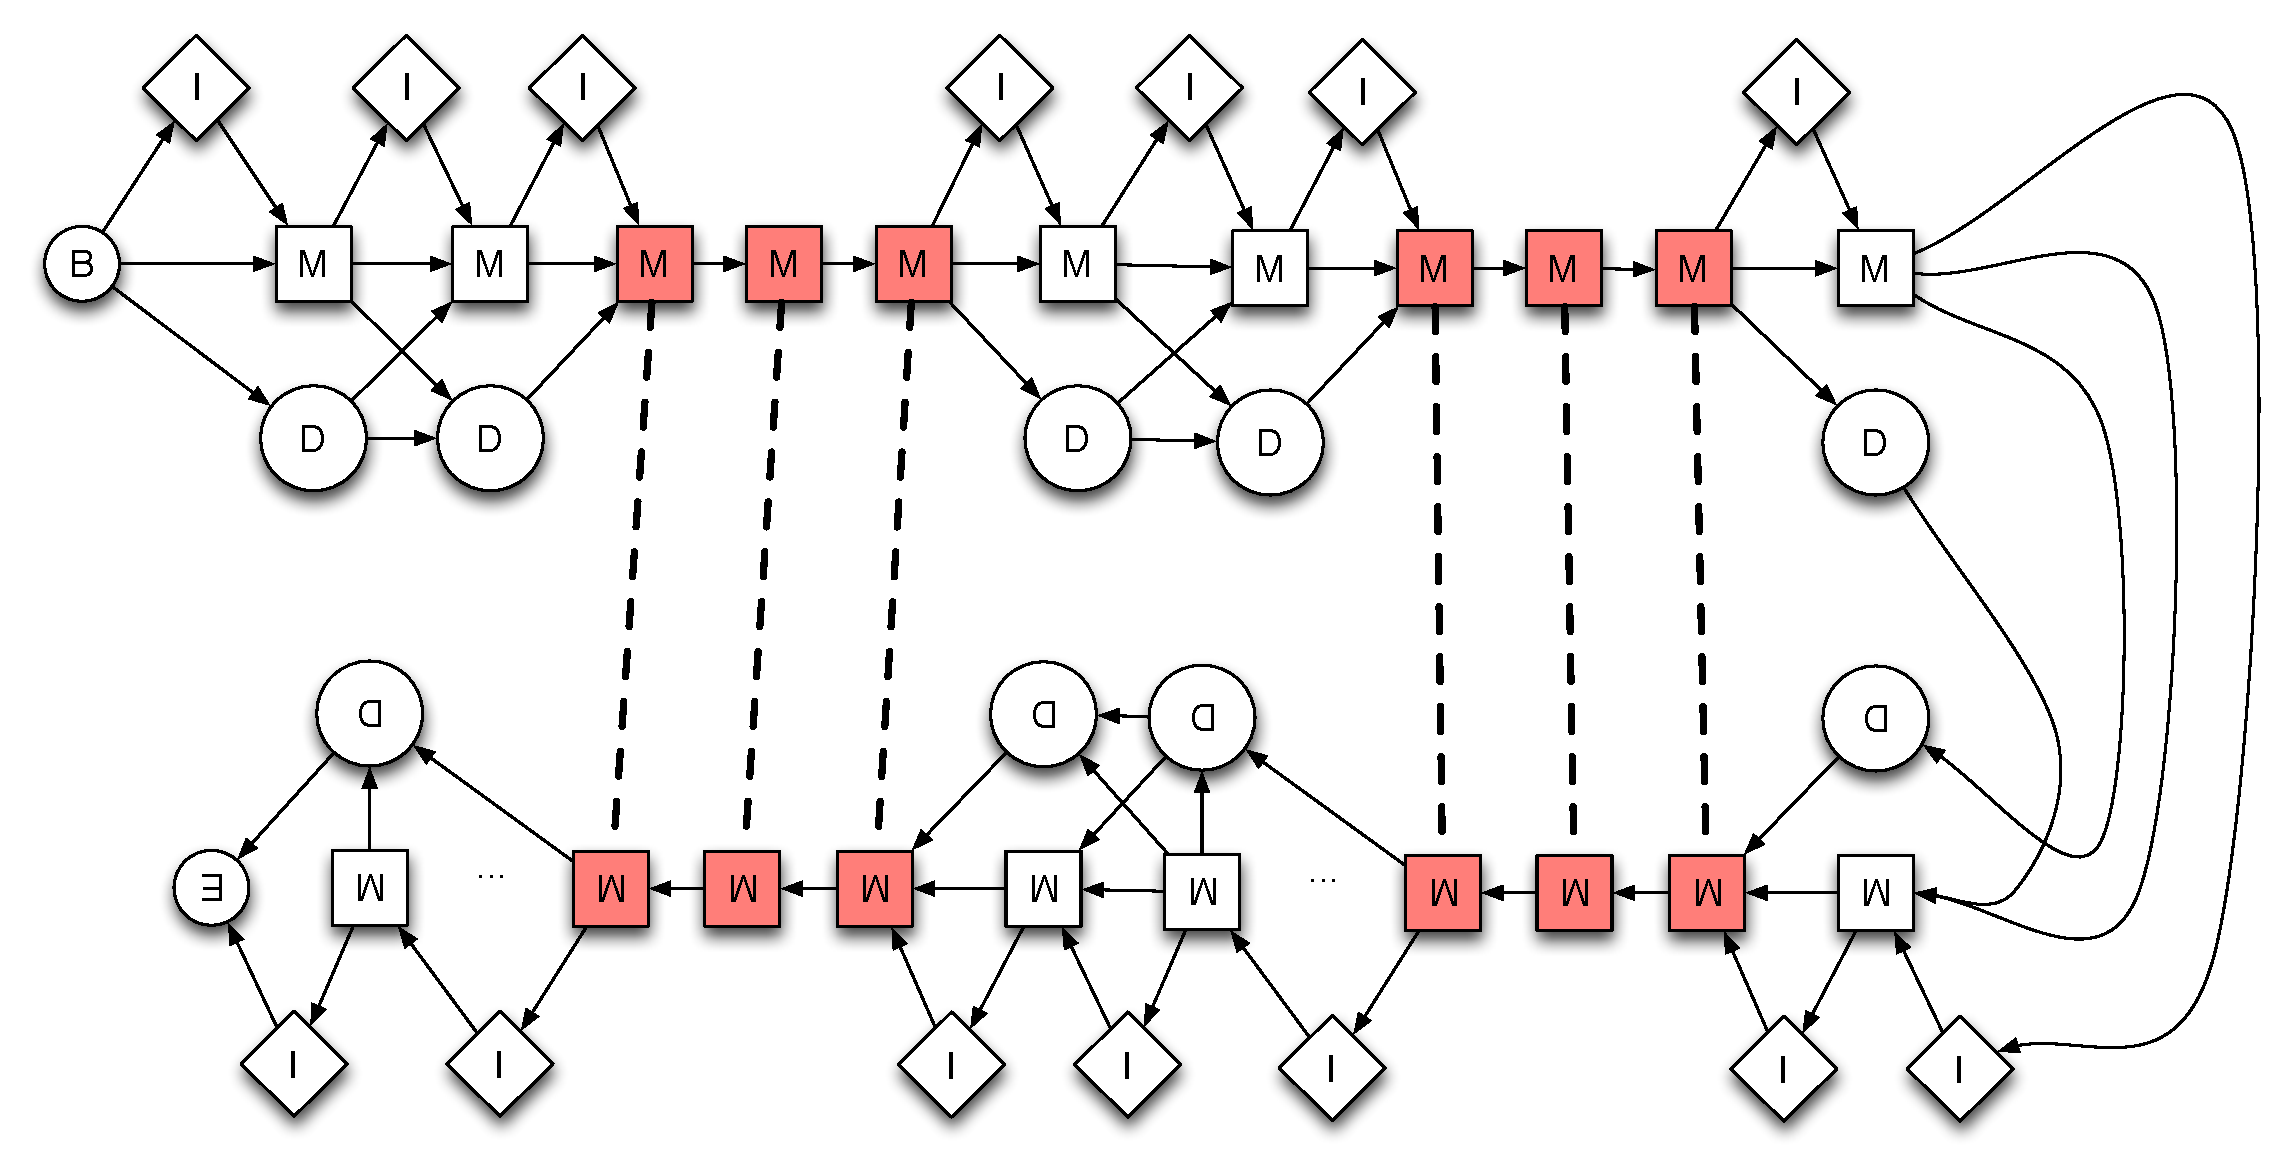
\includegraphics[width=8cm]{mrf_interleave_diagram.pdf}} 
\else
\centerline{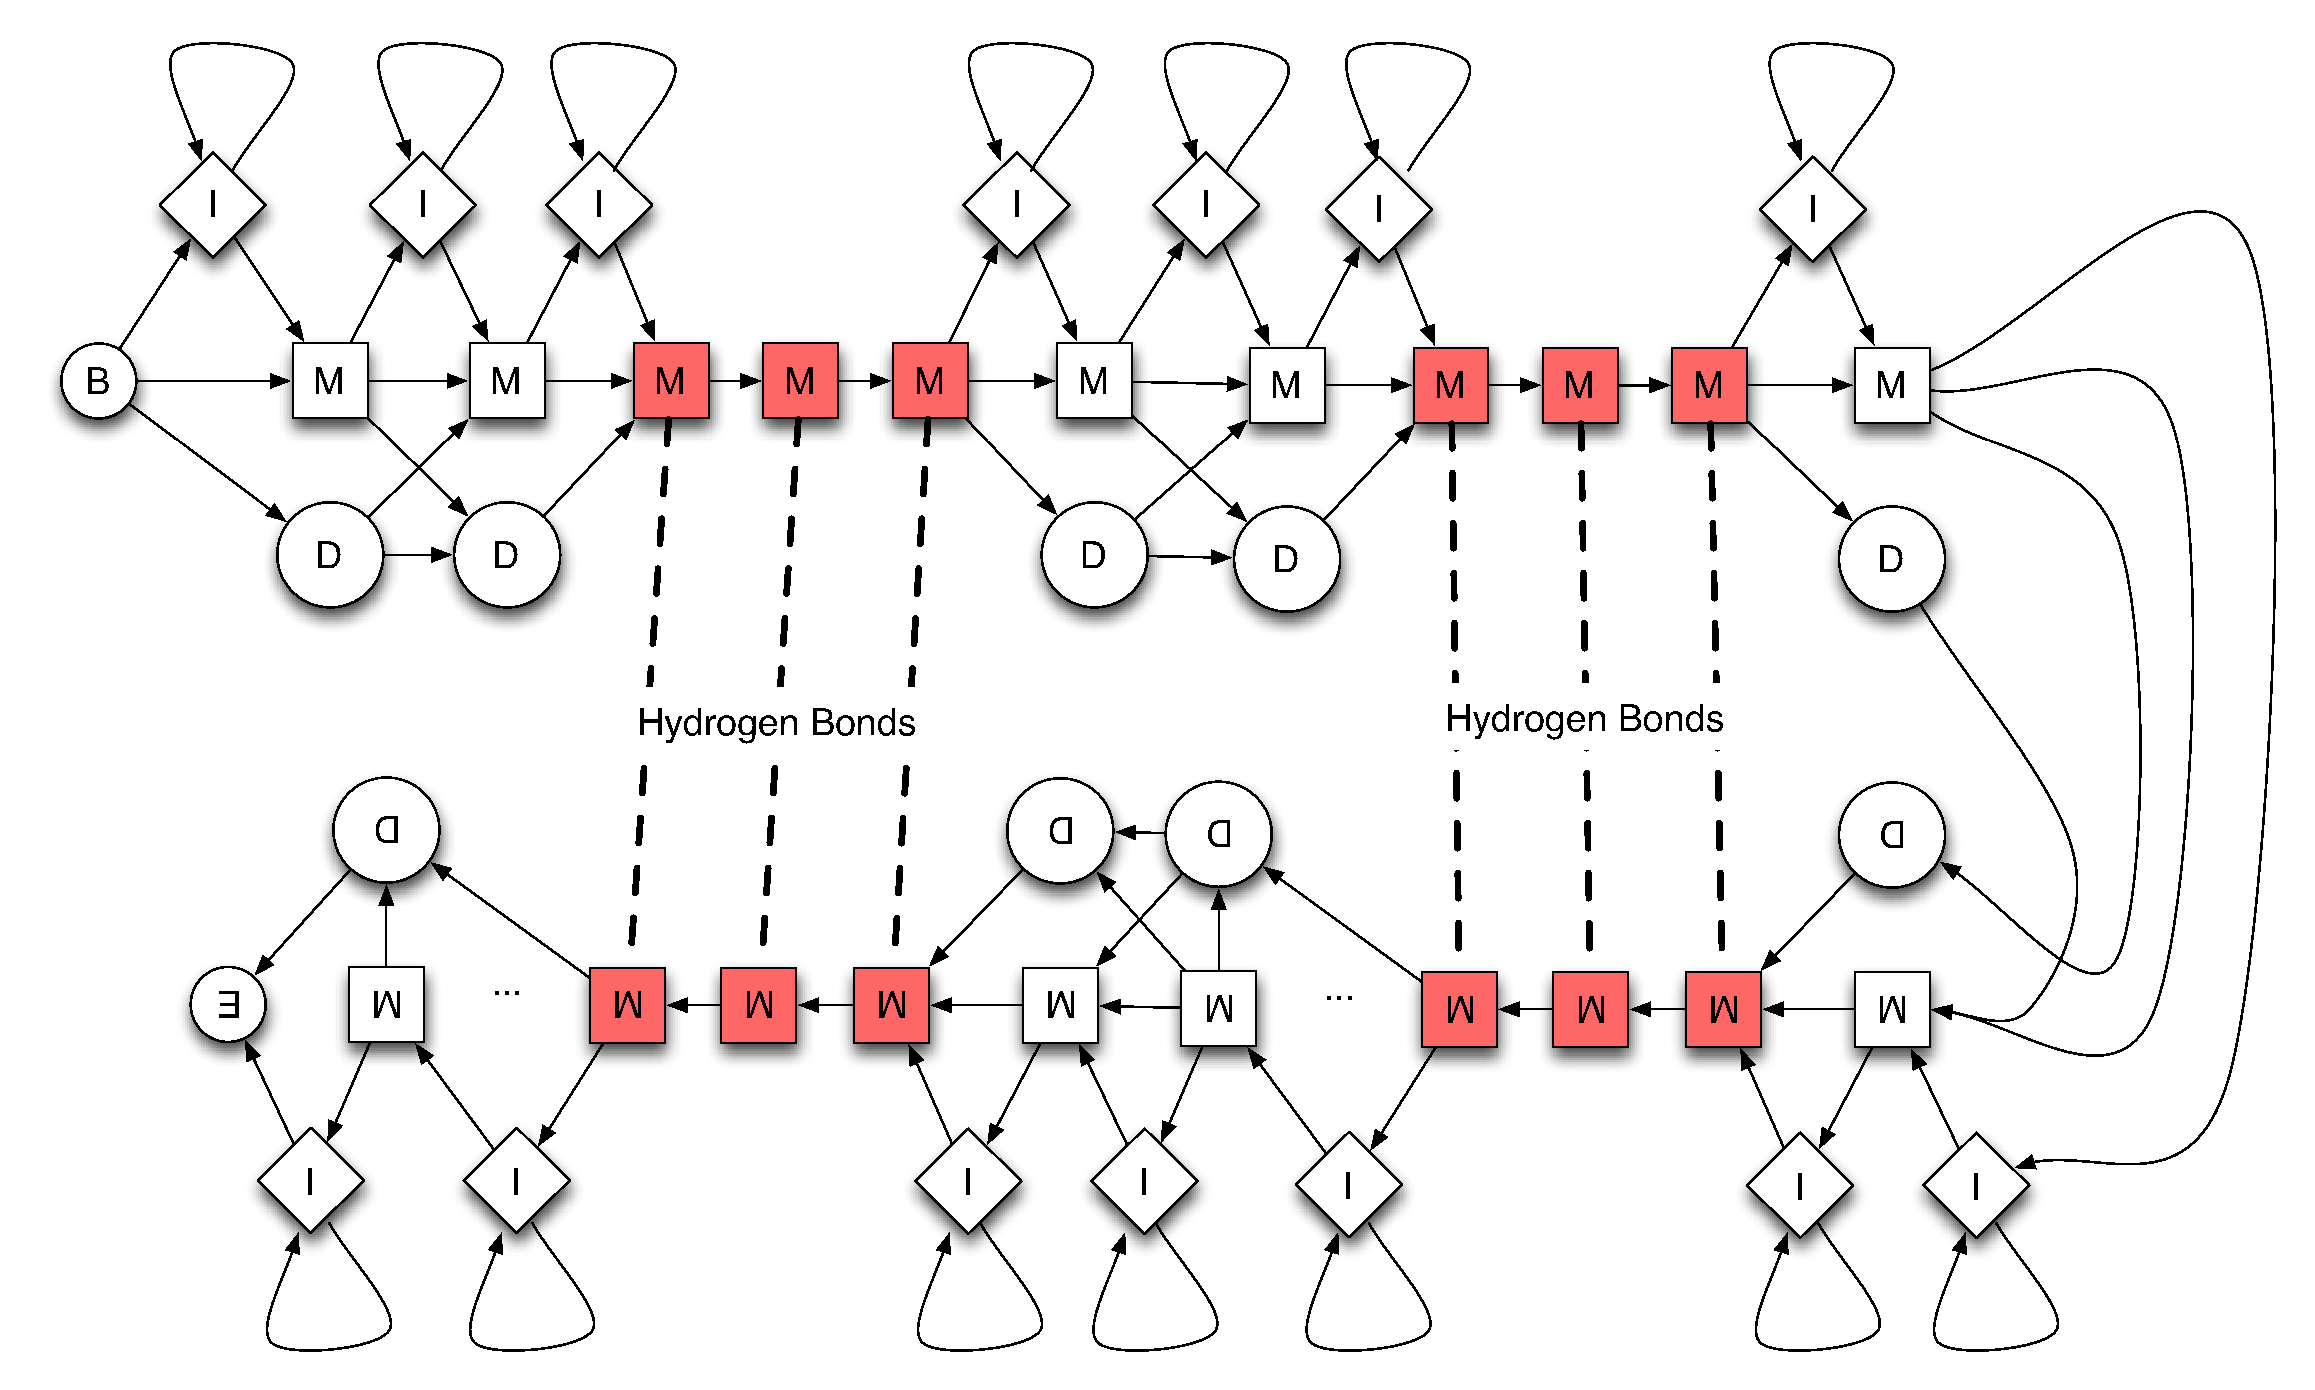
\includegraphics[width=8cm]{mrf_interleave_diagram.eps}} 
\fi
Each shaded node represents a beta-strand position.
Nodes connected by dashed edges are hydrogen-bonded.

\caption{A Markov random field with two beta-strand pairs}
\label{mrf} 
\end{figure}



We~address this problem by combining ``generate and filter'' into a
single abstraction, which has type \mono{SearchGen pt r}.
Type variable~\texttt{pt} is a point in the search
space, and \texttt{r} is a
random-number generator.
\mono{Rand~r} is a lazy monad of stochastic computations:
\smallverbatiminput{gen.tex}
The monadic computation \texttt{pt0} randomly selects a starting point
for search;
\texttt{nextPt} produces a new point from
an existing point.
Because scoring can be expensive, both \texttt{pt0}
and \texttt{nextPt} use \emph{scored} points, and they can
reuse scores from previous points.

To tell if a point returned by \texttt{nextPt} is useful, we call
 the \texttt{utility} function,
which scrutinizes a move represented as follows:
\smallverbatiminput{move}
The decision about utility uses not only a source of randomness but
also the \emph{cumulative cost} of the point, which we define to be
the number of points explored previously.
The~cumulative cost of the current point is also the age of the
search,
and
in~simulated annealing, for example, as the search ages,
the \texttt{utility} function becomes less likely to accept a move
that worsens the score.

\noindent
\vbox{
Using these pieces, function \texttt{everyPt} produces an infinite
sequence containing a mix of useful and useless moves:
\smallfuzzverbatiminput{10.8pt}{everygen}
}
\noindent
Both \texttt{nextPt} and \texttt{utility} are monadic, but 
we can still use a little bit of
laziness:
from its starting point, \texttt{everyPt} produces an infinite list of
randomly chosen successor points, then calls \texttt{costedUtility} to
tag each one with a cumulative cost and a utility.
We~hope that if you look carefully at how \texttt{successors} is computed,
you will understand why we
separate \texttt{pt0}~from~\texttt{nextPt} instead of using a single
function that produces an infinite list:
We~don't \emph{want} the infinite list that would result from
applying \texttt{nextPt} to many points in succession;
we~want the infinite list that results from applying \texttt{nextPt}
to \texttt{startPt} many times in succession, each time with a
different source of randomness.

Once the successors have been computed and tagged,
\texttt{span} finds the first useful successor.
In~case there \emph{is} no successor, \texttt{everyPt} also returns
all the useless successors.
If~we do find a useful successor, we start searching anew from that
point, with a recursive call to \texttt{everyPt}.
(Because \texttt{everyPt} is monadic, the points accumulated so far are
appended to its result using the \verb+<$>+~operator.)
%
The most informative part of \texttt{everyPt} is last expression of
the \texttt{do} block,
which shows that the result begins with a useful point,
is followed by a (possibly infinite, possibly empty) list of useless
points, and then continues recursively with the results of \texttt{everyPt}.

The rest of the search uses Hughes's
classic composition of generator  and test function.
Because our code is monadic, we~use the monadic composition
operator~\texttt{=<<}, which is the bind operator with its arguments
swapped: 
\smallverbatiminput{search}
The \texttt{test} function has type \mono{SearchStop~pt}:\\
\smallverbatiminputx{stop}
Type \mono{History~pt} retains only the useful points.
(Internally, \mrfy\ needs only the \emph{final} useful point,
but because we want to study how different search algorithms behave,
we~keep all the useful points.)

The definition of \texttt{SearchStop} reveals two forms of
non-modularity which are inherent in \mrfy's search algorithm.
First, we need \texttt{Utility} because if we omit the useless states,
search might not terminate.
Second, we need \texttt{CCosted} because some of our test functions
decide to terminate based either on the cumulative cost of the most
recent point or on the difference between costs of successive useful points.

Despite these non-modular aspects, the search
interface provides ample scope for
experiments.
Random hill climbing took 50~lines of code and one~day to
implement.  
Simulated annealing requires only a new
\texttt{utility} function, which took 15~lines of code and half an hour to implement.
(Hill climbing accepts a point if and only if it scores better than its
predecessor;
simulated annealing may accept a point that scores worse.)
Our genetic algorithm reuses the same
\texttt{pt0} and \texttt{SearchStop} functions, and its \texttt{utility}
function took only a few lines of code.
\remark{This claim isn't supported by inspection of the code.}
But~the recombination of parent
placements in its \texttt{nextPt} function took forty lines of code
and a full day to implement.

We're not entirely happy with the way we're writing individual
functions.
In~particular, \texttt{SearchStop} functions aren't composable;
we~can't, for example, combine two functions to say that we'd like to
stop if scores aren't improving or if we've tried a thousand points,
whichever comes first.
Eventually, we'd like to have
combinator libraries for \texttt{SearchStop} and \texttt{nextGen}, at~least.

%%  Our \texttt{SearchStrategy} interface somewhat resembles an object-oriented
%%  style of programming.
%%  However, it is \textit{easier} to create a SearchStrategy
%%  in Haskell than using conventional object-oriented techniques, because
%%  all the functions in a SearchStrategy are partial applications of
%%  other functions.
%%  If we were using conventional object-oriented
%%  techniques, we would have to declare subclasses with instance
%%  variables and would have to write code to initialize objects of those
%%  subclasses. 


\subsection{Performance}

\seclabel{perf}
\seclabel{performance}

At each point in its search,
MRFy calls \verb+vee'+ several
 times.
Our~\verb+vee'+
function computes a \mbox{\mono{Scored [StateLabel]}}, that~is, 
an~optimal path and its score.
But at intermediate points in \mrfy's search,
\mrfy\ uses only the
score.
Even though Haskell evaluation is lazy, \verb+vee'+ 
still allocates thunks that could compute paths.
To~measure the relevant overhead,
we~cloned \verb+vee'+ and modified it to compute
only a score, with no path.
This change improved 
run time by nearly~50\%.
%%But when \texttt{search} finally decides on a placement, we need a
%%version of \verb+vee'+ that \emph{does} compute a path, so we can
%%extract the optimal parse for that placement.

How could we keep the improvement without 
maintaining two versions of \verb+vee'+?
In~Lisp or Ruby we would have used macros or metaprogramming,
but we were not confident of our ability to metaprogram a solution
using Template Haskell.
Instead, we use higher-order functions.
As~shown in \secref{vee-prime},
\verb+vee'+ does not use primitive~\primcons\ but instead
uses an unknown function \texttt{cons}, which is
passed~in.
To~get a path, we pass in primitive~\primcons;
to~get just a score, we pass in
\verb+\_ _ -> []+.
This trick is simple and easy to implement, and it provides the same
speedup as the cloned and modified~code.
But~we have an uneasy feeling that it may work only because of
undocumented properties of GHC's inliner, which may 
change without warning. 

Even with this trick,
MRFy's implementation of Viterbi's algorithm is much
slower than the C++ version implemented in \mrfy\'s predecessor,
SMURF.
For example, on a micro-benchmark that searches for a
structural motif of 343 nodes in a protein of 2000 amino acids,
\mrfy\ takes 2.32~seconds and
SMURF takes 0.29~seconds.

But \mrfy's job is not to run Viterbi's algorithm on large models;
\mrfy's job is to detect homologies to structures on which Viterbi's
algorithm is intractable.
We~benchmarked \mrfy\ 
using a model of an ``8-bladed beta propeller,''
which has 343 nodes, of which 178 appear in 40~beta strands.
The models between beta strands typically have at most 10~nodes.
We~used a query sequence of 592 amino acids, but each placement breaks
the sequence into 41~pieces, each of which typically has at most 20 amino
acids.
CAN WE PLEASE REPLACE THE TEXT ABOVE WITH A DESCRIPTION OF WHAT'S
GOING ON IN THE CODE WE ACTUALLY RAN???
On~these smaller problems, 
performance is good enough that \mrfy\ can do its job.
%%
%%
%%
SUDDEN CHANGE OF BENCHMARK CONSIDERED HARMFUL.
%%
%%
Given a Markov random field with a 12-stranded ``beta sandwich''
structure,
\mrfy\ typically computes an alignment within a minute;
SMURF allocates over 16GB of memory
and does not terminate even after eight hours.

Because \mrfy\ works on many subproblems independently, we~found it easy
to improve performance through parallelism.
Calls on query sequences between beta strands are independent,
as are calls on different placements.
Using
\texttt{Control.Parallel}, parallelizing this computation was as easy
as  substituting
\texttt{parmap rseq} for \texttt{map}.
On a 48-core, 2.3GHz AMD Opteron 6176 system, 
parallel performance is good up to about 12~cores.
\figref{fig:efficiency} shows parallel efficiency when
using a model of an ``8-bladed beta propeller;''
the model has 165 ordinary nodes and 40~beta strands totalling
178 nodes.
We~benchmarked \mrfy\ using a query sequence of
592 amino acids.
Figure~\ref{fig:speedup} SHOWS NOTHING OF VALUE BECAUSE RANDOMNESS
BREAKS EVERYTHING.  AND IT SHOULD HAVE ERROR BARS.
(Parallel efficiency is 1.0 when the speedup is equal to the number of cores
used.
Lower speedups mean lower efficiency.)


%%  \begin{figure}[h!]
%%  \centerline{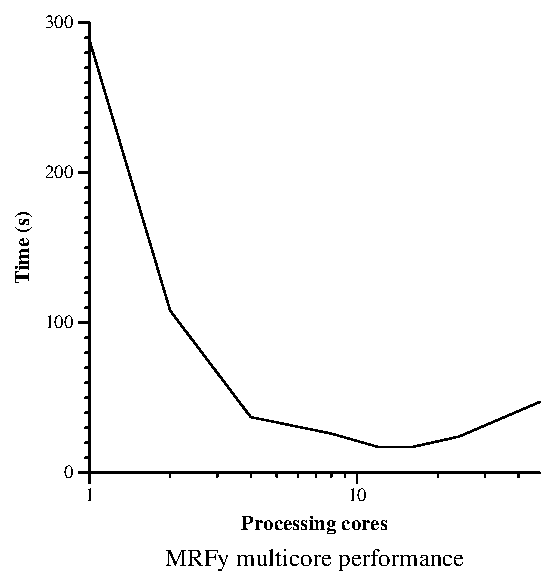
\includegraphics[width=6cm]{mrfy_multicore_log}}
%%  \caption{MRFy run-time performance with varying
%%  numbers of processing cores on a large protein}
%%  \label{multicore}
%%  \end{figure}


\begin{figure}%%%[h!]
\centerline{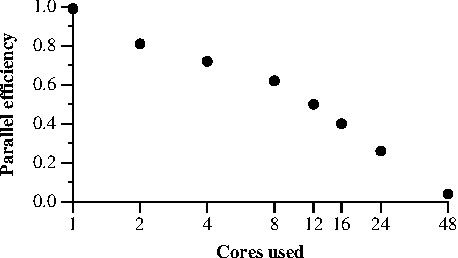
\includegraphics{efficiency}}
\bigskip
\caption{\mrfy's WRONG parallel efficiency}
\label{fig:efficiency}
\end{figure}

%%% Had we implemented the SMURF algorithm in Haskell, we believe that performance
%%% would be unacceptable.
%%% However, for the algorithm underlying MRFy, we are satisfied with the runtime
%%% performance of Haskell and GHC.
%
% Nonetheless, we expect that we can still improve MRFy's run-time performance
% with further profiling and tuning.  
% And we expect that if we cross the street, we will get to the other side.





\subsection{Awkward debugging and testing}

\seclabel{awkward-profiling}

We've shown you some of the code we like, but we've also written 
code we dislike.
The~code we like least is what we've written to work around
obstacles we 
encountered in debugging.

We hate the code we've written to help debug
run-time errors.
Our~group's legacy file
format is poorly documented: when beta
strands overlap and are doubly paired, the invariants of the
format are not clear.
This format is hard to deal with no matter what
programming language is used, and faults are to be expected.
But using Haskell, we had a hard time diagnosing run-time errors.
Calls to
\texttt{trace} 
littered our code,
even when relegated to wrapper functions.
We~weren't aware of the backtrace feature of GHC's profiler,
and even after we discovered that feature, it didn't help:
the profiler can be used only on very small test cases that didn't always trigger
run-time errors.
This same limitation affected the GHCi debugger; 
in~GHCi, our \texttt{vee'} function
is too slow to be runnable on nontrivial
inputs.
Moreover, the GHCi debugger can set breakpoints only at top-level functions
or at specific column/line positions, which made debugging the memoized
\texttt{vee''} function impractical.
In~August 2011, 
Lennart Augustsson said that the biggest advantage of Strict
Haskell is getting a stack trace on error,
and Simon Marlow said that he may have figured out how to track call
stacks properly in a lazy functional language.
We~can't wait.

Our difficulties with debugging led to internal disagreements.
The~junior members of our team wanted to apply the debugging
skills they had honed through years of imperative programming.
These skills did not transfer well to Haskell.
The senior member of the team kept saying that any proper approach to
debugging Haskell code should involve QuickCheck.
This exhortation was unhelpful.

\seclabel{awkward-quickcheck}

Only the senior member of our team was able to use
QuickCheck easily.
In~retrospect, we~have identified some obstacles that prevented the
junior people from using
QuickCheck.
\begin{itemize}
\item
The examples and tutorials we found focused 
predominantly on writing and testing properties using data types that
already implemented class \texttt{Arbitrary}.
We~didn't understand the \texttt{Arbitrary} class very well, 
perhaps because the overloaded \texttt{arbitrary} value is not a
function.
For programmers accustomed to object-oriented dispatch
on \emph{arguments}, it is hard to grasp how Haskell's type-class
system can find the proper version
of \texttt{arbitrary}.
\item
Our difficulties were compounded by a weak understanding of monads.
We~were too baffled by QuickCheck's \texttt{Gen} monad to grasp its
importance.
\item
We~continually overlooked the critical role of \emph{shrinking}.
As~a result, on the one or two occasions we did 
use QuickCheck, the counterexamples were too large to be
informative. 
\end{itemize}
Because of these obstacles, 
we wrote thousands of lines of code without ever defining an instance
of \texttt{Arbitrary} and therefore
without looking hard at QuickCheck.
After the fact, we were overwhelmed by the work
involved in writing and testing instances
of
\texttt{Arbitrary}.
The work got done only because the whole team got involved in order to
meet the deadlines for this paper.

Based on the QuickCheck properties we did write, we have identified and
easily fixed a bug in our implementation of Viterbi's algorithm; we had not
been including the score for the transition from the final node of the hidden
Markov model to the special ``end'' state.
Without QuickCheck, it is unlikely that we would have found this bug,
and if we had, determining the cause would have required much time.

%%  At~that point, we were quickly about to write QuickCheck
%%  specifications for several properties of the Viterbi algorithm:
%%  \begin{itemize}
%%  \item
%%  The total number of \verb+Mat+ and \verb+Ins+ states returned equals
%%  the number of amino acids in the query sequence.
%%  \item
%%  The total number of matches, and deletions returned equals the
%%  number of nodes in the hidden Markov model,
%%  \emph{except} that an initial sequence of
%%  of~\verb+Ins+ states counts as a single node,
%%  due to an odd property of the HMMER file format (namely, the zeroth
%%  node has no delete state and a non-emitting match state which
%%  is always occupied, but a normal insert state).
%%  \item
%%  The sequence returned satisfies the Plan7 invariant, that is, states
%%  \verb+Ins+ and \verb+Del+ are never adjacent.
%%  \end{itemize}
%%  \textbf{These properties need to be followed by more ambitious
%%  properties},


 
 
\section{Our previous experience compared}
\seclabel{comparo}

Our Haskell code for hidden Markov models and Viterbi's algorithm
solves the same problems as existing C++~code.
Other researchers using Haskell may also have to reimplement code,
but researchers may also reimplement code out of choice, not
necessity.
In computational biology, reimplementing existing algorithms is unremarkable.
For~example, both SMURF and HMMER contain new implementations of these
same algorithms.
In~MRFy, we are using the Haskell implementations to help solve new
problems. 

When performance has mattered, members of our group, like other
computational biologists, have used~C++.
To~compare our Haskell experience with our C++ experience,
we discuss three tools:
\begin{itemize}
\item
Matt~\cite{Menke:2008wu} is used to create alignments like that shown
in \figref{alignment}.
It~comprises about 12,000 lines of~C++.
The only external tools or libraries it uses are \texttt{zlib}
and \texttt{OpenMP}, and its initial development took two years.
\item
SMURF
\cite{Menke:2010ti} is used to detect homologous proteins in the presence
of paired beta strands.
It~comprises about 9,000 lines of~C++, of which about 1,000~lines are
shared with~Matt.
It~uses no external tools or libraries, and
its initial development took a year and a half.
It uses multidimensional dynamic programming to exactly compute the alignments
for which MRFy relies on stochastic search.
As a result, in the presence of complex beta-strand topologies, SMURF is
computationally intractable.
\item
MRFy is used to detect homologous proteins in the presence of paired
beta strands; it effectively supplants SMURF.
It~comprises about 2300 lines of~Haskell, 300 of which are devoted
to tests and QuickCheck properties and generators.
Neither C++ codebase includes any testing facilities.
MRFy~uses several external tools and libraries, of which the most
notable are Parsec, the BioHaskell bioinformatics library, and
the libraries \path{Data.MemoCombinators}, \path{Control.Parallel},
and \path{Data.Vector}.
Its initial development took about three months.
%%%% \remark{Others were mostly full-time work, but no need to distinguish.}
\end{itemize}
Like much research software, all three of these tools were written
 in~haste.
We~have experience modifying the older tools.



We~modified Matt to use information about sequences as well as structure.
The modification added 2,000 lines of code, and it calls
external sequence aligners that we did not write.
We~thought the modification would take three months, 
but it took most of a~year.
Matt uses such
data structures as mutable oct-trees, vectors, and arrays.
It~uses clever pointer arithmetic.
The mutable data structures were difficult to 
repurpose, and the pointer arithmetic was \emph{too} clever: 
nearly every change resulted in new segfaults.

We~had hoped to extend Matt further, with support for partial alignments,
which we~expected to require only 
a cosmetic manipulation of the 
output.
But
this feature wound up
requiring deep information about Matt's data structures,
and we had to give~up.
We~believe we could write an equivalent tool in~Haskell,
with most of Matt's performance, in at most nine months.

Our most painful experience was adding ``simulated evolution''
to~SMURF \cite{Daniels:2012}. 
Although simulated evolution represents a relatively minor
enhancement,
just understanding the existing code took several months.

We~built MRFy quickly, and we expect that
higher-order functions will make MRFy easy to extend.
Each new addition to MRFy's stochastic search has taken at most a day
to implement.

Haskell encourages hasty programmers to slow down.
We~have to get the types right,
which makes it hard to write very large functions.
To~get the code to typecheck, we~have to write type signatures, which
also serve as documentation.
And once the types are accepted by the compiler,
it~is not much more work to write contracts for important functions.
MRFy is still hasty work.
Many types could be simplified;
we're~sure we've missed opportunities for abstraction;
and we know that MRFy's decomposition into modules could be improved.
But despite being hasty programmers, we produced code 
that is easy to understand and easy to extend.
Our hastily written Haskell beats
our hastily written Ruby and~C++.


Looking beyond our research group to computational biology more
broadly, our experience with other software is better.
Little of it is written in functional languages, 
but much of the software shared by the community is excellent.
MRFy's training component was derived from that of~HMMER,
and
working with the HMMER 
codebase was pleasant;
data structures and their
mutators are well documented. 
There is a 
BioHaskell library, part of which we use,
but it is not nearly as 
complete as BioPython or BioRuby, which are heavily used in the community.
We hope that tools for computational biology in
Haskell continue to mature. 

\section{What can you learn from our experience?}

If~you are a computational biologist, 
you can be productive in Haskell without extensive preparation.
Two~of us (Daniels and Gallant) are graduate students.
Daniels has taken a graduate seminar in functional programming, which
included some Haskell;
Gallant has taken a programming-languages course which included
significant functional programming but no Haskell.
Ramsey is a professor who has used Haskell 
for medium-sized projects,
but his contributions to MRFy have been limited, mostly to \emph{post hoc}
refactoring and testing.


\subsection{Obstacles to be overcome}

GHC's profiler assigns costs not to functions but to ``cost
centers'' \cite{sansom-pj}.
In GHC~7.0, which we used 
for most of MRFy's development, 
cost-center annotations can be added automatically only
to top-level 
functions.
But most of our code is in nested functions.
We~annotated such functions manually,
but the annotations
made our code so ugly that we felt compelled to
remove them as soon as possible.
Without the annotations, however, GHC's call-site and allocation
profiles did not give us enough information to be useful.
We~miss valgrind, whose profiler gives useful information
without \emph{any} annotations.
GHC~7.4 provides much
better profiling tools, which eliminate most of these obstacles,
rendering this experience no longer as relevant.

Like other functional programmers, we~have found that 
once we have our types right, our code is often right.
But~MRFy computes with arrays and array indices,
and in that domain, types don't help much.
Bounds violations lead to run-time errors, which we have not been able
to identify any systematic way to~debug.
GHC's profiler can provide stack traces, but we~found this information
difficult to discover, and as noted above,
there are obstacles to profiling.
We're~aware that debugging lazy functional programs has been a topic
of some research,
but one of the biggest obstacles we encountered to using Haskell is
that we have had to abandon our old approaches to debugging.

Ideally we would use QuickCheck to find bugs, but as we mention in
\secref{awkward-quickcheck}, we found obstacles.
We~have now overcome these obstacles, but
we~sorely regret not doing so earlier.
In~light of our experience, we will institute a new programming practice:
whenever we introduce a new data type,
we~will write the instance of
\texttt{Arbitrary} right away, while
relevant invariants are still fresh in memory.
When invariants are not enforced by Haskell's static type system,
we~will write them as Haskell predicates.
We can then immediately run QuickCheck on each predicate, to verify
that our Arbitrary instance agrees with the predicate.
For each predicate~\texttt{p} we can also check
\mono{fmap (all p . shrink) arbitrary}.






\subsection{Information that will help you succeed}

If~you want to use Haskell in your research, we~believe that you must
have enough experience with functional programming that you can build
\emph{all} the code you need, not only the code that is easy to write
in a functional language.
Implementing Viterbi's equations in Haskell was pure joy.
Writing an iterative search in purely functional style was~easy.
Transforming data in the HMMER file format, \emph{without}
using mutable state the way the C++ code does, was difficult.

\seclabel{penumbra}

While the Haskell community offers many
enticing tools, libraries, and packages,
be aware that
not all of them are worth using.
Some are not ready for prime time, and some were once great but are
no~longer maintained.
The great packages, like \texttt{Data.MemoCombinators} and Parallel
Strategies, are truly great.
But~for amateurs, it's not always easy to tell the great packages from the wannabes
and the has-beens.
And even some of the great packages could be better documented, with
more examples.

%%  Most of the software we used came from Hackage, which is the Haskell
%%  community's software repository.
%%  We~sometimes found it hard to tell
%%  if a particular Hackage package was right for us.
%%  In particular, as beginning 
%%  functional programmers, we~found some documentation inaccessible.
%%  The documentation that we found most accessible typically contained
%%  examples showing how to use a particular tool or library.
%%  \remark{So what's our message here? What are we telling people to
%%  think or do differently? ---NR}


As~in any endeavor, access to experts helps.
We~would have been better off if our in-house expert had been an
enthusiastic student and not a busy professor.
But we have been surprised and pleased by the help available from
faraway experts on Stack Overflow and on Haskell mailing lists.
Although a local expert makes things easier, one is not
 absolutely necessary.

\section{Conclusion}

A~little knowledge of and a lot of love for functional programming
enabled us to carry out a successful research project in a language
that computational biologists seldom use.
If~you \emph{want} to use Haskell---or one of your graduate students
wants to use Haskell---you can
succeed. 




% - No obvious body of knowledge on code improvement. 
%  

 

\acks

Anonymous referees spurred us to think
more deeply about laziness and to write more carefully about performance.
Josef Svenningsson suggested a correspondence between \mrfy's search
and stream fusion, which led us eventually to the \texttt{Utility} type.
Koen Claessen instantly diagnosed an inappropriately strict
implementation of the \texttt{Rand} monad.
We also thank Lenore Cowen, Kathleen Fisher, Ben Hescott, Brad
Larsen, and Nathan Ricci. 


\bibliographystyle{simplenat}

% The bibliography should be embedded for final submission.

\bibliography{mrfy_experience_report}

\iffinaldraft


\vfill

\begingroup
\parfillskip=0pt
\advance\leftskip by 0pt plus 30em
\emph{You can live to surf the Haskell wave, but~if you slide off the crest, you
drown.}
\par
\endgroup

\fi

%%%%    \break
%%%%    
%%%%    
%%%%    \appendix
%%%%    
%%%%    
%%%%    \section{Orphaned text}
%%%%    
%%%%    
%%%%    In~our C++ work, the faults we encounter most frequently are
%%%%    segmentation faults, 
%%%%    memory errors caused by pointer arithmetic or uninitialized 
%%%%    memory,
%%%%    and heap exhaustion.
%%%%    In~our Haskell work, the faults we encounter most frequently are
%%%%    type errors and bounds-checking errors in array and vector accesses.
%%%%    While we have found the bounds-checking errors difficult to debug,
%%%%    they are less difficult than memory errors.
%%%%    
%%%%    
%%%%    Implementing the equation in this form was not only intellectually
%%%%    satisfying; it~also helped us find
%%%%    bugs.
%%%%    The most memorable bug was that in one of our base cases, 
%%%%    we~mistakenly returned an empty path of states;
%%%%    the correct result was a singleton path containing the initial state.
%%%%    Very quickly after observing a missing state in the output, we were
%%%%    able to find the faulty case in the code.
%%%%    
%%%%    
%%%%    

\break


\begin{figure}%%%[h!]
\centerline{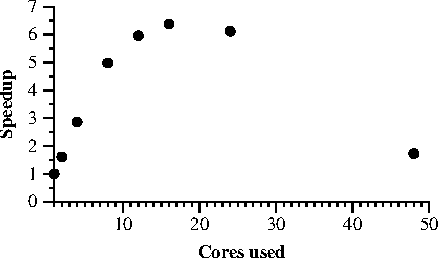
\includegraphics{speedup}}
\bigskip
\caption{\mrfy's parallel speedup}
\label{fig:speedup}
\end{figure}




\end{document}
